% Declare the overview figure before the result text so it stays beside the results.
\begin{revadded}
\begin{figure*}[t]
\centering
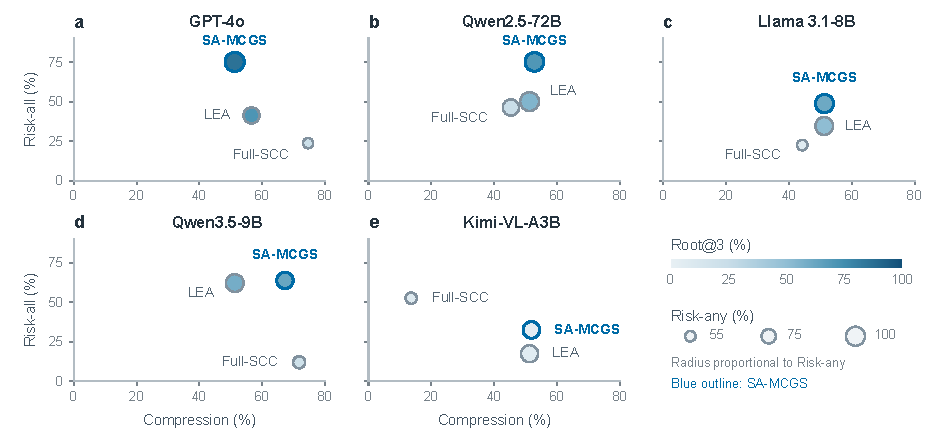
\includegraphics[width=\textwidth]{figures_equal_budget_20261012/equal_budget_tradeoff.pdf}
\caption{Five-backbone comparison with SA-referenced baseline budgets. Position shows compression and \riskall{}; bubble radius is proportional to \riskany{}, and fill color encodes \rootthree{} (0--100\%). Blue outlines mark historical \samcgs{} outputs.}
\label{fig:equal_budget_tradeoff}
\end{figure*}
\end{revadded}

% Main comparison: locked values in ARR_OCT2026_MASTER_REVISION_PLAN_ZH.md, Section 4.2.
% September 25 table remains green; October 1 compressed result prose is red.

\revreplace{\samcgs{} achieves higher \rootthree{} than both One-shot and LEA on GPT-4o, Qwen2.5-72B, Llama 3.1-8B-Instruct, and Qwen3.5-9B (Table~\ref{tab:matched_main}). The largest gain over LEA is 17.50 percentage points on Llama 3.1-8B-Instruct.

Complete risk-evidence retention also improves: \riskall{} increases by 31.25 percentage points over LEA on GPT-4o and Qwen2.5-72B, and by 13.75 on Llama 3.1-8B-Instruct. On Gemini 2.5 Pro, all three methods achieve \riskall{} between 83.75\% and 85.00\%.

On Qwen3.5-9B, \samcgs{} combines higher \rootthree{} with 67.25\% compression, matching LEA's \riskall{} of 63.75\%.}{\samcgs{} improves \rootthree{} over both baselines on four of the five backbones, with the largest gain over LEA on Llama 3.1-8B-Instruct (17.50 percentage points; Table~\ref{tab:matched_main}). It improves \riskall{} over LEA by 31.25 points on GPT-4o and Qwen2.5-72B, and by 13.75 on Llama. On Gemini 2.5 Pro, all three methods achieve \riskall{} between 83.75\% and 85.00\%.}


\revadd{Over five fixed backbones, mean \riskall{} improves by 15.25 points over LEA (95\% source-SCC bootstrap interval: 2.00--27.75); the \rootthree{} interval includes zero ($-0.25$--14.00). Resampling preserves source-level dependencies (Appendix~\ref{app:main_confidence_intervals}).}
